\documentclass[a4]{article}
\usepackage{amssymb}
\usepackage{amsmath}
\usepackage{bm}
\usepackage{graphicx}

\DeclareMathOperator*{\argmax}{argmax}
\DeclareMathOperator*{\argmin}{argmin}



\newtheorem{defn}{Definition}

%opening
\title{ Notes on Latent Direchlet Allocation with Full Bayesian Treatment }
\author{Shoichiro Yamanishi}

\begin{document}

\maketitle

%\begin{abstract}
%\end{abstract}


\section{Overview}
This is an expository document for latent Direchlet allocation in the full Bayesian setting
for $\beta$ matrix.
This is an outcome of my own self study into the original article, and it has turned out to be
a very good streamlined study material for EM-algorithm and variational Bayes worth documenting by myself for
my own better understanding.

The main purpose of this document is to quickly and effortlessly refresh my memory in the future
as my own memory aid.

Another purpose is to fill the gap between the original article\cite{NIPS2001_2070} and the blog articles
available on Internet. The original article is too terse, and it takes me a lot of paper-and-pencil work
to comprehend the contents.
It also briefly touches on the full Bayesian treatment. On the other hand, the blog
articles focus on a quick grasp of the concept with rich illustrations, and rigorous
mathematical treatment is usually ommitted.

This document is characterized as follows.
\begin{itemize}
\item Comprehensive math treatment from the modeling down to just before implementation for both training and inference.
\item Full-bayesian $\beta$ with prior $\eta$.
\item Small gaps between two adjacent equations through the course of deductions at the cost of lengthiness.
\item Discussion on possibility of treatment of using the columns of $\beta$ as word embeddings with non-informative priors.
\end{itemize}


This document is organized as follows. First, the generative model is defined,
and then the problems of the training and the inference are defined.
Then the training problem is solved by a version of EM-algorithm.
First the expectation part of finding the posterior distribution is approximated by
variational Bayes, specifically by the mean field approximation.
And then the training parameters $\bm{\alpha}$ and $\eta$ are updated in the maximization step.
The maximization of those parameters are solved by Newton-Raphson method and it is then explained.
Solving Newton-Raphson method involves evaluating Digamma and Trigamma functions, and 
numerical approximation techniques are explained.
Finally, a possibility of using the columns of $\beta$ as word embeddings in relation to 
the topic inference of a new document with non-informative priors is explained.





%//////////////////////////////////////////////////////////////////////////////////////
%                        section Generative Model Formation
%//////////////////////////////////////////////////////////////////////////////////////





\section{Generative Model Formation}
Latent Direchlet allocation is a generative probabilistic model proposed by \cite{NIPS2001_2070} for documents
utilizing something called exchangeability of words in a document 
(de Finetti's Theorem). It is also used to generate word embeddings, notably lda2vec\cite{DBLP:journals/corr/Moody16}.

\begin{defn}
$\mathbf{w}_n$ represents a word for the $n$-th position of a document.
It is a one-of-$V$vector such that $\mathbf{w}_n \in \{0,1\}^V$ where always only one
element is 1, and the rest is 0. We use the notation $w^v_n = 1$ 
if $w_n$ represents the $v$-th word, or $w^v_n = 0$ if $w_n$ does not 
represent the $v$-th word,
\end{defn}

\begin{defn}
$W_m = (\mathbf{w}_{m1}, \mathbf{w}_{m2},\cdots, \mathbf{w}_{mN_{m}})$
represents a document. It is an ordered list of $N_m$ words.
\end{defn}

\begin{defn}
$\mathcal{D} = \{ W_1, W_2,\cdots, W_M\}$ represents a corpus.
It is a set of $M$ documents.
\end{defn}

The aim of this model is to represent a document $W_m$ by 
{\bf a probability distribution} $\bm{\theta}_m$ of $K$ topics.
Naturally it is a multinomial distribution.
It is drawn from a Dirichlet prior $\bm{\alpha} \in \mathcal{R}^K$,
which is learned empirically.

\begin{equation}
\begin{aligned}
p( \bm{\theta}_m | \bm{\alpha} )
    = Dir( \bm{\theta}_m | \bm{\alpha} )
    = \frac{  \Gamma( \sum_k \alpha_k )  }
           { \prod_k \Gamma(\alpha_k)    }
      \prod_{k=1}^K ( \theta_m^k )^{\alpha_k - 1}\label{p(theta_m|alpha)}
\end{aligned}
\end{equation}

where $0 \le \theta_m^k \le 1$ denotes the $k$-th element of the vector
$\bm{\theta}_m$.
Please note that $\bm{\theta}_m$ itself represents a multinomial probability
distribution.

In LDA, each word $\mathbf{w}_{mn}$ in a document $W_m$ is drawn from a 
distribution in $\beta$, which is dictated by a latent variable 
$\mathbf{z}_{mn}$, which is a one-of-$K$ vector drawn from $\bm{\theta}_m$.
This means the model assigns a topic for each word $\mathbf{w}_{mn}$, and it 
can be different for each word in a document.

Once the topic for $\mathbf{w}_n$ is determined by $\mathbf{z}_{mn}$ as $k$,
then the word assignment (which $v$ of $V$ is assigned) is drawn from a 
probability distribution $\beta_{[k:*]}$. $\beta$ is a $K \times V$ matrix, 
and $\beta_{[k:*]}$ represents a multinomial distribution for topic $k$.
Each $\beta_{[k:*]}$ is drawn from a common uniform Direchlet prior $\eta$.
Here we denote the row $\beta_{[k:*]}$ by a vector $\mathbf{b}_k$
and  $0 \le b_k^v \le 1$ denotes the $v$-th element of the vector
$\mathbf{b}_k$ for notational convenience.

\begin{equation}
\begin{aligned}
p( \mathbf{b}_k | \eta )
    = Dir( \mathbf{b}_k | \eta )
    = \frac{ \Gamma( V \eta )  }
           { \Gamma(\eta)^V    }
      \prod_{v=1}^V ( b_k^v )^{\eta - 1}\label{p(b_k|eta)}\\
\end{aligned}
\end{equation}

$\bm{\alpha}$ and $\eta$ are learned empirically using a version of EM.
The model for a document $W_m$ is expressed as a marginalization of the joint
distribution
$p(W_m, \bm{\theta}_m, Z_m, \beta | \bm{\alpha}, \eta )$
over $\bm{\theta}_m$, $Z_m$, $\beta$ where
$Z_m = (\mathbf{z}_1, \mathbf{z}_2, \cdots, \mathbf{z}_{N_m})$ as follows.
The joint distribution is:
\begin{equation}
\begin{aligned}
p( W_m, \bm{\theta}_m, Z_m, \beta | \bm{\alpha}, \eta ) 
    &= p( \bm{\theta}_m | \bm{\alpha} )
       \prod_{k=1}^{K} \left( p( \mathbf{b}_k | \eta ) \right )
       \prod_{n=1}^{N_m} \left( 
           p( \mathbf{z}_{mn} | \bm{\theta}_m          )
           p( \mathbf{w}_{mn} | \mathbf{z}_{mn}, \beta )
       \right)\\
    &= Dir( \bm{\theta}_m | \bm{\alpha} )
       \prod_{k=1}^{K} \left( Dir( \mathbf{b}_k | \eta ) \right)
       \prod_{n=1}^{N_m} \left(
           \prod_{k=1}^{K}
               (\theta_m^k)^{z_{mn}^k} 
               (b_k^{v_{mn}})^{z_{mn}^k} 
       \right) \label{p(W_m,theta_m,Z_m,beta|alpha,eta)}\\
\end{aligned}
\end{equation}
where ${z_{mn}^k} \in \{0,1\}$ denotes the $k$-th element of 
the vector $\mathbf{z}_{mn}$, and $v_{mn}$ denotes the 
column in $\beta$ ($v_{mn}$-th element of the vector $\mathbf{b}_k$)
 such that $(\mathbf{w}_{mn})^{v_{mn}} = 1$.
And the marginalized ditribution for $W_m$ is:
\begin{equation}
\begin{aligned}
p(W_m | \bm{\alpha}, \eta)
   &= \int_{|\mathbf{b}_1| = 1,\: 0 \le \mathbf{b}_1 \le 1}
      \int_{|\mathbf{b}_2| = 1,\: 0 \le \mathbf{b}_2 \le 1}
      \cdots
      \int_{|\mathbf{b}_K| = 1,\: 0 \le \mathbf{b}_K \le 1}\\
   &\:\:\:\:\int_{|\bm{\theta}_m|=1,\: 0 \le \bm{\theta}_m \le 1} 
      \sum_{Z_{m}} p( W_m, \bm{\theta}_m, Z_m, \beta | 
      \bm{\alpha}, \eta ) d\bm{\theta}_m
      d\mathbf{b}_K \cdots d\mathbf{b}_2 d\mathbf{b}_1\label{p(W_m|alpha,eta)}\\
\end{aligned}
\end{equation}
where the summing over $Z_{m}$ indicates all the possible $K^{N_m}$ 
combinations of
$Z_{m} = (\mathbf{z}_{m1}, \mathbf{z}_{m1}, \cdots, \mathbf{z}_{N_m} )$.
Clearly this summation itself is already intractable.
The corpus is modeled as follows.
\begin{equation}
\begin{aligned}
p( \mathcal{D} | \bm{\alpha}, \eta ) 
    &= \prod_{m} p( W_m | \bm{\alpha}, \eta )\label{p(D|alpha,eta)}\\
\end{aligned}
\end{equation}
The equation \ref{p(D|alpha,eta)} is the basis for the EM algorithm assuming
each document $\mathbf{w}_m$ is i.i.d.


\begin{figure}
\centering
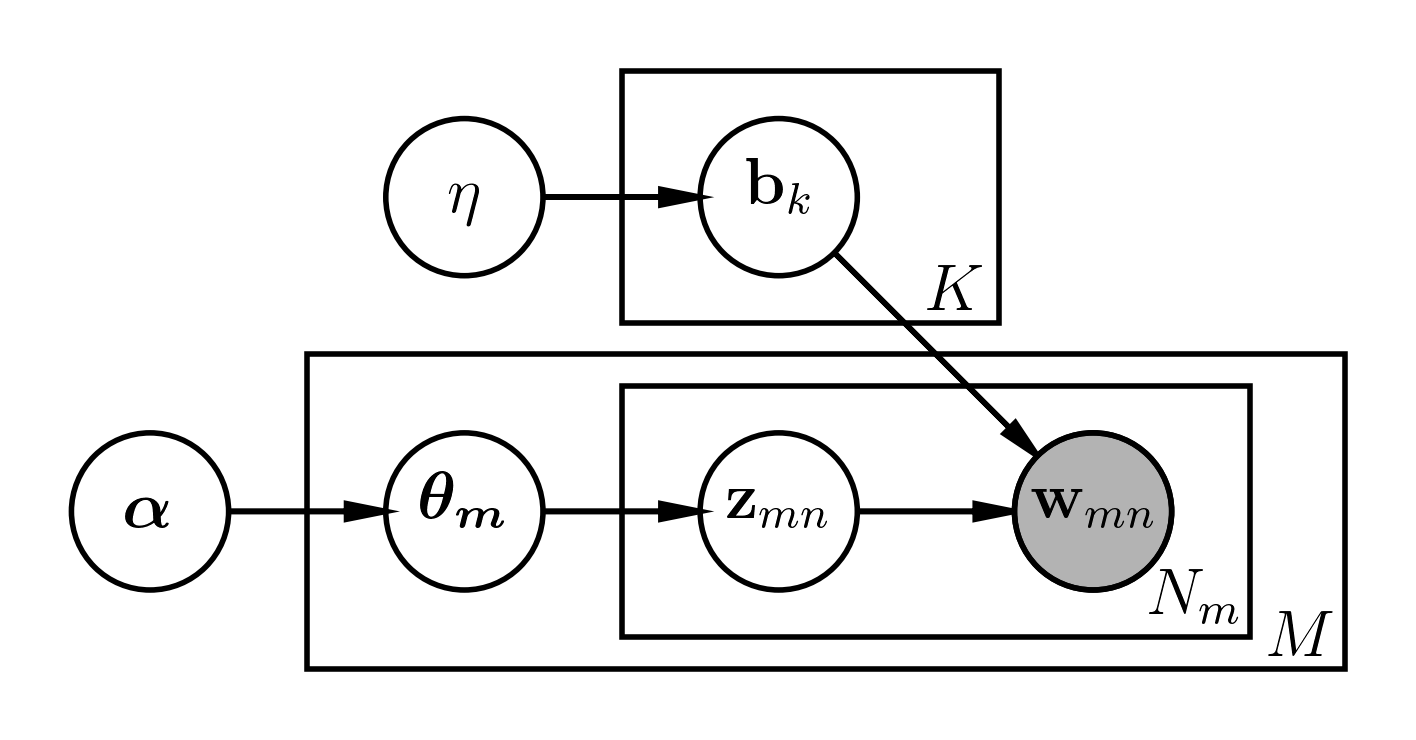
\includegraphics[width=8cm]{lda_modelling.png}
\caption{Generative Model}
\label{fig:generative model}
\end{figure}


%//////////////////////////////////////////////////////////////////////////////////////
%                             training and inference
%//////////////////////////////////////////////////////////////////////////////////////


\section{Training and Inference}
Basically we employ empirical Bayes in which we use MLE to learn 
$\bm{\alpha}$ and $\eta$ from the data.
We define \begin{bf}training\end{bf} as the point estimate of $\bm{\alpha}$ and $\eta$ such that
the posterior is maximized in MLE for the observed $\mathcal{D}$.

\begin{equation}
\begin{aligned}
\bm{\alpha}_{max}, \eta_{max} &= \underset{\bm{\alpha},\eta}{\mathrm{argmax}} \left( \ln p( \mathcal{D} | \bm{\alpha}, \eta ) \right)\\
&= \underset{\bm{\alpha},\eta}{\mathrm{argmax}} \left( \sum_{m=1}^M
\ln p( W_m, \bm{\theta}_m, Z_m, \beta | \bm{\alpha}, \eta ) 
\right)\\
&= \underset{\bm{\alpha},\eta}{\mathrm{argmax}} \Big( \sum_{m=1}^M \Big(
      \int\cdots\int\int
      \sum_{Z_{m}} \ln p( W_m, \bm{\theta}_m, Z_m, \beta | 
      \bm{\alpha}, \eta ) d\bm{\theta}_m
      d\mathbf{b}_K \cdots d\mathbf{b}_1
\Big)\Big)\label{MLE_alpha_eta}\\
\end{aligned}
\end{equation}

This is not a tractable problem and we use an EM algorithm in which
$\bm{\theta}_m$, $Z_m$, and $\beta$ are treated as latent variables.
For the EM-algorithm, we define the evidence lower bound as follows.

\begin{equation}
\begin{aligned}
ELBO_m = \mathbb{E}_{\bm{\theta}_m, Z_m, \beta \sim q_m(\bm{\theta}_m, Z_m, \beta)}
[\ln p( W_m, \bm{\theta}_m, Z_m, \beta | \bm{\alpha}, \eta ) - \ln q_m(\bm{\theta}_m, Z_m, \beta)]
\label{ELBO_m}\\
\end{aligned}
\end{equation}
where $q_m(\bm{\theta}_m, Z_m, \beta)$ is a certain joint probability distribution for 
$\bm{\theta}_m$, $Z_m$, and $\beta$.
\subsection{E-step}
In the E-step of the normal EM algorithm, we identify
$q_m(\bm{\theta}_m, Z_m, \beta)$ with the posterior with certain fixed 
$\bm{\alpha}^*$ and $\eta^*$.

\begin{equation}
\begin{aligned}
q_m^{*}(\bm{\theta}_m, Z_m, \beta) &= 
\underset{ q_m(\bm{\theta}_m, Z_m, \beta) }
{\mathrm{argmax}} ( ELBO_m )\\
&= p( \bm{\theta}_m, Z_{m}, \beta | W_m, \bm{\alpha}^*, \eta^* )\label{normal_EM_conditional}\\
\end{aligned}
\end{equation}
However as we later explain, $p( \bm{\theta}_m, Z_{m}, \beta | W_m, \bm{\alpha}^*, \eta^* )$ is still intractable, and
we need an approximation of it. One way of approximation is to use variational mean field approximation by breaking
conditional dependences among $\bm{\theta}_m$, $Z_m$, and $\beta$. This is further explained in the following section.


\subsection{M-step}
In the M-step we raise $ELBO_m$ w.r.t. $\bm{\alpha}$ and $\eta$ with fixed $q_m^{*}(\bm{\theta}_m, Z_m, \beta)$.

\begin{equation}
\begin{aligned}
\bm{\alpha}^*, \eta^* &= \underset{\bm{\alpha},\eta}{\mathrm{argmax}} \left( \sum_m ELBO_m \right)\\
&= \sum_m \mathbb{E}_{\bm{\theta}_m, Z_m, \beta \sim q^*_m(\bm{\theta}_m, Z_m, \beta)}
[\ln p( W_m, \bm{\theta}_m, Z_m, \beta | \bm{\alpha}, \eta ) - \ln q^*_m(\bm{\theta}_m, Z_m, \beta)]\\
&= \sum_m \mathbb{E}_{\bm{\theta}_m, Z_m, \beta \sim q^*_m(\bm{\theta}_m, Z_m, \beta)}
[\ln p( W_m, \bm{\theta}_m, Z_m, \beta | \bm{\alpha}, \eta ) ]\label{M_step}\\
\end{aligned}
\end{equation}
The RHS of equation \ref{M_step} is concave in terms of $\bm{\alpha}$, $\eta$, and this is solved by taking the
derivative of it.

\begin{equation}
\begin{aligned}
\nabla_{\bm{\alpha}, \eta} \left( \sum_m
\mathbb{E}_{\bm{\theta}_m, Z_m, \beta \sim q^*_m(\bm{\theta}_m, Z_m, \beta)}
[\ln p( W_m, \bm{\theta}_m, Z_m, \beta | \bm{\alpha}, \eta ) ]\label{derivative_M_step}\right) = 0\\
\end{aligned}
\end{equation}

\subsection{Topic Vector and Per-topic Word Probability Distribution}
After the training has converged, we have the following, which together maximize $\sum ELBO_m$:
$\bm{\alpha}^*$, $\eta^*$, $q^*(\bm{\theta}_m)$ \& $q^*(Z_m)$ for each $W_m$, and $q^*(\beta)$.
$q^*(\bm{\theta}_m)$ can be considered a topic vector for the document $W_m$, 
$q^*(Z_m)$ is further factorized into $\prod_{n=1}^{N_m} q^*(\mathbf{z}_{mn})$ and 
$q^*(\mathbf{z}_{mn})$ is considered a word-level topic vector, which can also be considered a 
document-dependent word embedding.
$q^*(\beta)$ is further factorized into $\prod_{k=1}^{K} q^*(\mathbf{b}_{k})$ and each 
$q^*(\mathbf{b}_{k})$ can be considered the probability distribution over all the words for that topic.

\subsection{Topic Inference for a New Document}
We define \begin{bf}inference\end{bf} of a new Document $W_{new}$ as finding $q^{max}(\bm{\theta}_{new}, Z_{new})$ such
that $q^{max}(\bm{\theta}_{new}, Z_{new})$ maximizes $ELBO_{new}$ for the fixed $\bm{\alpha}$ and $\eta$ as well as 
$q^*(\beta)$. This is solved by the mean value approximation, and it is further explained in the following section.
$q^{max}(\bm{\theta}_{new})$ can be considered the infered topic.

As a single point estimate, we can apply MAP on $q(\bm{\theta})$.
In fact, as explained in the subsection \ref{approximator_theta_m},
$q(\bm{\theta})$ is formed as $Dir( \bm{\theta} | \bm{\gamma} )$ and 
$\bm{\gamma}$ is numerically computerd. Then we can find the mode as follows.
\begin{equation}
\begin{aligned}
\theta_{MAP}^k = \frac{\gamma^k - 1}{\sum_{j=1}^K \gamma^j - K  }
\end{aligned}
\end{equation}
However, the original article \cite{NIPS2001_2070} simply suggests to use $\bm{\gamma}$ as the topic vector.


\begin{figure}
\centering
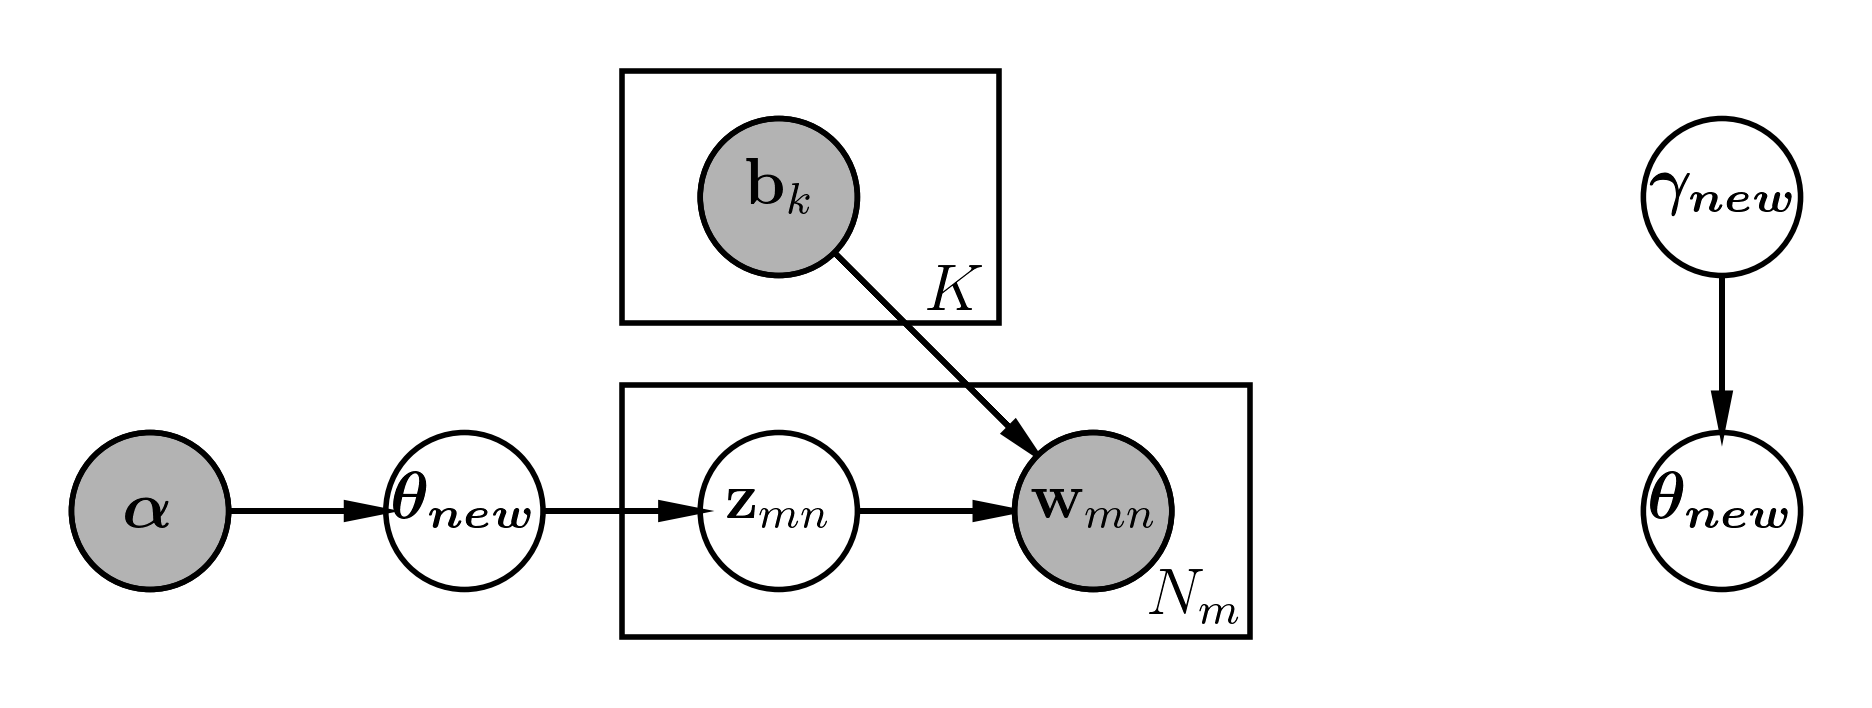
\includegraphics[width=8cm]{lda_inference.png}
\caption{Infering $\theta_{new}$. The left side is the modeling and the right side is the approximation of $\theta_{new}$}
\label{fig:lda_inference}
\end{figure}





%//////////////////////////////////////////////////////////////////////////////////////
%                          section Variational E-Step
%//////////////////////////////////////////////////////////////////////////////////////



\section{
    Variational E-Step
}\label{variational E-step}
This is the inner loop of the algorithm for approximating the posterior with the variational mean field approximation
EM requires to represent the terms with
    $\bm{\theta}_m$, $Z_m$, and $\beta$
in equation \ref{model_w} in the expectation of the following conditional distribution. 
\begin{equation}
\begin{aligned}
p( \bm{\theta}_m, Z_{m}, \beta | W_m, \bm{\alpha}, \eta ) =
    \frac{ p( W_m, \bm{\theta}_m, Z_{m}, \beta | \bm{\alpha}, \beta ) }
         { \sum_{W_m} 
               p( W_m, \bm{\theta}_m, Z_{m}, \beta | \bm{\alpha}, \eta ) }
\label{EM_conditional}\\
\end{aligned}
\end{equation}
However, both LHS and the denominator of RHS are intractable.
Especially the denominator of RHS sums over all the elements of $W_{m}$,
whose number is $V^{N_m}$. It is not factorized per word $\mathbf{w}_{mn}$ due to
the explaining-away effect between $\mathbf{z}_{mn}$ for all $n$ and $\mathbf{b}_k$ for all $k$ conditioned on
$\mathbf{w}_{mn}$.
Therefore, an approximation of this is required. For that we use 
mean field approximation as follows.
\begin{equation}
\begin{aligned}
  p( \bm{\theta}_m, Z_{m}, \beta | \mathbf{w}_m, \bm{\alpha}, \eta )
  &\approx
      q(\bm{\theta}_m , Z_{m}, \beta )\\
  &= q( \bm{\theta}_m )
     \prod_{n = 1}^{N_m} q( \mathbf{z}_{mn} )
     \prod_{k=1}^{K} q( \mathbf{b}_k )\label{q_forEM}\\
\end{aligned}
\end{equation}
Please note that $q( \mathbf{b}_k )$ are not per-document, but corpus-wise approximators.

\subsection{Approximator $q( \bm{\theta}_m )$}\label{approximator_theta_m}

Since $0 \le \bm{\theta}_m \le 1$ is dictated by a Direchlet distribution,
we introduce a variational parameter $\bm{\gamma}_{m}$ such that 
$ q( \bm{\theta}_m ) = Dir( \bm{\theta}_m | \bm{\gamma}_{m} ) $.
The following holds from the properties of the Direchlet distribution.

\begin{equation}
    \mathbb{E}_{\bm{\theta}_m \sim Dir( \bm{\theta}_m | \bm{\gamma}_{m})}
        [\theta_m^i] = \frac{ \gamma_{m}^i }{ \sum_{k=1}^{K} \gamma_{m}^k }
\end{equation}

\begin{equation}
    \mathbb{E}_{ \bm{\theta}_m \sim Dir( \bm{\theta}_m | \bm{\gamma}_{m}) }
        [\ln(\theta_m^i)] =
            \Psi( \gamma_{m}^i ) - \Psi( \sum_{k=1}^{K} \gamma_{m}^i )
\end{equation}

where $\Psi(x) = \frac{d\Gamma(x)}{dx}$ is a Digamma function 
(the first derivative of the gamma function).
Digamma and Trigamma functions can be numerically computerd by approximation.


\subsection{Approximator $q( \mathbf{b}_k )$}

$0 \le \mathbf{b}_k \le 1$  is dictated by a Direchlet
distribution, and we introduce a variational parameter $\bm{\omega}_k$
such that $ q( \mathbf{b}_k ) = Dir( \mathbf{b}_k | \bm{\omega}_{k} ) $.

\begin{equation}
    \mathbb{E}_{\mathbf{b}_k \sim Dir( \mathbf{b}_k | \bm{\omega}_{k})}
        [b_k^v] = \frac{ \omega_{k}^v }{ \sum_{v=1}^{V} \omega_{k}^v }
\end{equation}

\begin{equation}
    \mathbb{E}_{ \mathbf{b}_k \sim Dir( \mathbf{b}_k | \bm{\omega}_{k}) }
        [\ln(b_k^v)] =
            \Psi( \omega_{k}^v ) - \Psi( \sum_{v=1}^{V} \omega_{k}^v )
\end{equation}

\subsection{Approximator $q( \mathbf{z}_{mn})$}

$\mathbf{z}_{mn}$ is a multinomial distribution,
we introduce a variational parameter
$\bm{\phi}_{mn} \in \mathcal{R}^K, |\bm{\phi}_{mn}| = 1$
,
$0 \le \bm{\phi}_{mn} \le 1$ 
such that
$q( \mathbf{z}_{mn}) = Mult(\mathbf{z}_{mn} |\
    \bm{\phi}_{mn}) = \prod_{k=1}^K (\bm{\phi}_{mn}^k)^{\mathbf{z}_{mn}^k}$.
The following trivially holds.
\begin{equation}
   \mathbb{E}_{ \mathbf{z}_{mn} \sim Multi (\mathbf{z}_{mn} |  \bm{\phi}_{mn})}
   [ \mathbf{z}_{mn} ]
   = \bm{\phi}_{mn}\\
\end{equation}

\subsection{Putting all the approximators together}

The equation \ref{q_forEM} is reformed as follows. 
\begin{equation}
\begin{aligned}
    q( \bm{\theta}_m , Z_{m}, \beta )
&=
    q(\bm{\theta}_m | \bm{\gamma} ) 
    \prod_{k=1}^{K} q(\mathbf{b}_k | \bm{\omega}_k ) 
    \prod_{n = 1}^{N_m}  q( \mathbf{z}_{mn} | \bm{\phi}_{mn} )\\
&=
    Dir(\bm{\theta}_m | \bm{\gamma} )
    \prod_{k = 1}^{K}Dir(\mathbf{b}_k | \bm{\omega}_k )
    \prod_{n = 1}^{N_m}  Mult( \mathbf{z}_{mn} | \bm{\phi}_{mn} )\\
&=
    Dir(\bm{\theta}_m | \bm{\gamma} )
    \prod_{k = 1}^{K}Dir(\mathbf{b}_k | \bm{\omega}_k )
    \prod_{n = 1}^{N_m} \prod_{v=1}^V (\phi_{mn}^v)^{z_{mn}^v}
    \label{q_forEM2}\\
\end{aligned}
\end{equation}


\begin{figure}
\centering
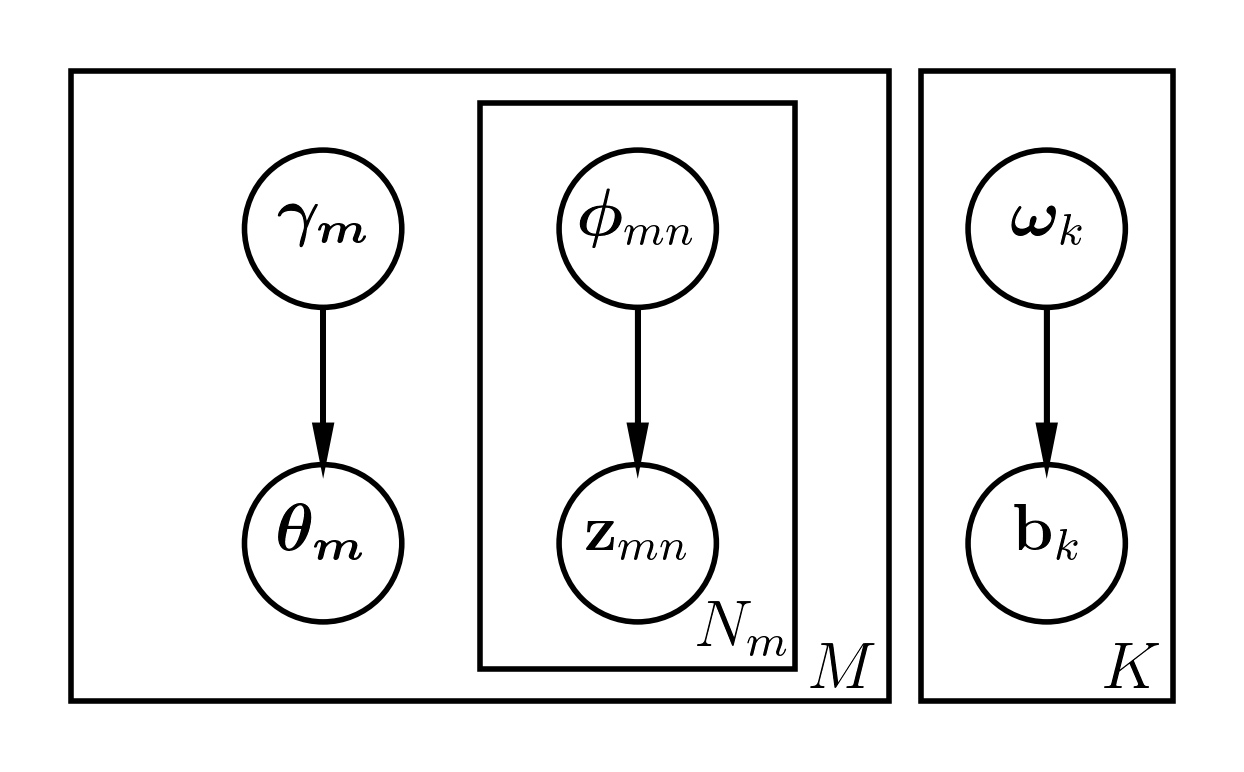
\includegraphics[width=6cm]{lda_approximation.png}
\caption{Approximator $q( \bm{\theta}_m , Z_{m}, \beta )$}
\label{fig:lda_approximation}
\end{figure}


\subsection{Evidence Lower Bound with the Approximators}
We form a variational ELBO for the observed document $W_{m}$ as follows.

\begin{equation}
\begin{aligned}
ELBO_m &= \mathbb{E}_{\bm{\theta}_m , Z_{m}, \beta \sim
                    q(\bm{\theta}_m , Z_{m}, \beta )}
            [    \ln p( W_m, \bm{\theta}_m, Z_m, \beta | \bm{\alpha}, \eta)
               - \ln q(\bm{\theta}_m , Z_{m}, \beta ) ]\label{elbo_m}\\
\end{aligned}
\end{equation}
The first term on the RHS of the equation \ref{elbo_m} will be:

\begin{equation}
\begin{aligned}
    ELBO_{pm}
    &=
    \mathbb{E}[\ln p( W_m, \bm{\theta}_m, Z_m, \beta | \bm{\alpha}, \eta )]\\
    &=
    \mathbb{E}\left[\:
       \ln Dir( \bm{\theta}_m | \bm{\alpha} ) +
       \sum_{k=1}^{K} \left( \ln Dir( \mathbf{b}_k | \eta ) \right) +
       \sum_{n=1}^{N_m}
           \sum_{k=1}^{K}
               z_{mn}^k \left( \ln \theta_m^k + \ln b_k^{v_{mn}} \right) 
       \:\right]\label{model_w}\\
    &=
      \ln \left( \Gamma( \sum_k \alpha_k ) \right) 
          - \sum_{k=1}^{K} \ln \Gamma(\alpha_k) 
          + \sum_{k=1}^{K} (\alpha_k - 1)
            \mathbb{E}_{\bm{\theta_m} \sim q(\bm{\theta_m)}}[\ln(\theta_m^k)]\\
      &\:\:\:\:+
      \sum_{k=1}^K \left(
          \ln \left( \Gamma( K\eta ) \right) 
          - K\ln \Gamma(\eta) 
          + \sum_{v=1}^{V} (\eta - 1) 
               \mathbb{E}_{\mathbf{b}_k \sim q(\mathbf{b}_k)}
               [\ln(b_k^v)]
      \right)\\
    &\:\:\:\:+
    \sum_{n=1}^{N_m} \sum_{k=1}^{K} 
        \mathbb{E}_{\mathbf{z}_{mn} \sim q(\mathbf{z_{mn}})} [z_{mn}^{k}] 
        \left(   \mathbb{E}_{\bm{\theta_m} \sim q(\bm{\theta_m)}}
                 [\ln \theta_m^k] 
               + \mathbb{E}_{\mathbf{b}_k \sim q(\mathbf{b}_k)}
                 [\ln b_{k}^{v_{mn}}] \right)\\
\end{aligned}
\end{equation}
where we used the assumed independence of the approximator as follows.
\begin{equation}
\begin{aligned}
\mathbb{E}_{ \mathbf{z}_{mn}, \bm{\theta_m} \sim 
    q(\mathbf{z}_{mn})q(\bm{\theta_m)} }
        [z_{mn}^{k} \ln \theta_m^k] 
=
    \left( \mathbb{E}_{\mathbf{z}_{mn} \sim q(\mathbf{z}_{mn})}
        [z_{mn}^{k}] \right)
    \left( \mathbb{E}_{\bm{\theta}_m \sim q(\bm{\theta}_m)}[\ln \theta_m^k]
    \right)\\
\end{aligned}
\end{equation}

\begin{equation}
\begin{aligned}
\mathbb{E}_{ \mathbf{z}_{mn}, \bm{\mathbf{b}_k} \sim 
    q(\mathbf{z}_{mn})q(\mathbf{b}_k)}
        [z_{mn}^{k} \ln b_m^k] 
=
    \left( \mathbb{E}_{\mathbf{z}_{mn} \sim q(\mathbf{z}_{mn})}
        [z_{mn}^{k}] \right)
    \left( \mathbb{E}_{ \mathbf{b}_k \sim q( \mathbf{b}_k) } [ \ln b_k^v ]
    \right)\label{elbo_pm}\\
\end{aligned}
\end{equation}

The second term on the RHS of the equation \ref{elbo_m} will be:
\begin{equation}
\begin{aligned}
    ELBO_{qm}
    &= - \mathbb{E}\left[\ln q(\bm{\theta}_m , Z_{m}, \beta)\right]\\
    &= - \mathbb{E}\left[
        \ln Dir(\bm{\theta}_m | \bm{\gamma} )
        + \sum_{k = 1}^{K} \ln Dir(\mathbf{b}_k | \bm{\omega}_k )
        + \sum_{n = 1}^{N_m} \sum_{v=1}^V {z_{mn}^v} \ln \phi_{mn}^v
       \right]\\
    &=
      - \ln \left( \Gamma( \sum_k \gamma_{m}^k ) \right) 
          + \sum_{k=1}^{K} \ln \Gamma(\gamma_{m}^k) 
          - \sum_{k=1}^{K} (\gamma_{m}^k - 1)
            \mathbb{E}_{\bm{\theta_m} \sim q(\bm{\theta_m)}}[\ln(\theta_m^k)]\\
      &\:\:\:\:+\sum_{k = 1}^{K} \left(
      - \ln \left( \Gamma( \sum_v \omega_k^v ) \right) 
          + \sum_{v=1}^{V} \ln \Gamma(\omega_k^v) 
          - \sum_{v=1}^{V} (\omega_k^v - 1)
            \mathbb{E}_{\mathbf{b}_k \sim q(\mathbf{b}_k)}[\ln(b_k^v)]
      \right)\\
      &\:\:\:\:-\sum_{n = 1}^{N_m} \sum_{k=1}^K
          \mathbb{E}_{z_{mn} \sim q(z_{mn})}[z_{mn}^k] \ln \phi_{mn}^k\label{elbo_qm}\\
\end{aligned}
\end{equation}


\subsection{Raising ELBO by Finding a Better $q(\bm{\theta}_m , Z_{m}, \beta )$}
Now we have formed $ELBO = ELBO_{pm} + ELBO_{qm}$ in terms of the expectations.
We are ready to raise ELBO in turn for each of $q(\bm{\theta}_m)$, 
$q(\mathbf{z}_{mn})$, and $q(\mathbf{b}_{k})$.


\subsubsection{Finding a Better $q(\bm{\theta}_m)$}
First we raise ELBO in terms of $q(\bm{\theta}_m)$.
For that we gather the relevant terms in ELBO into the following.

\begin{equation}
\begin{aligned}
    \mathcal{L}_{q(\bm{\theta}_m)}
    &= \sum_{k=1}^{K} (\alpha_k - 1)
       \mathbb{E}_{\bm{\theta_m} \sim q(\bm{\theta_m)}}[\ln(\theta_m^k)]\\
    &\:\:\:\:+
    \sum_{n=1}^{N_m} \sum_{k=1}^{K} 
        \mathbb{E}_{\mathbf{z}_{mn} \sim q(\mathbf{z_{mn}})} [z_{mn}^{k}] 
        \left(
            \mathbb{E}_{\bm{\theta_m} \sim q(\bm{\theta_m)}} [\theta_m^k] 
        \right)\\
    &\:\:\:\:
      - \ln \left( \Gamma( \sum_k \gamma_{m}^k ) \right) 
      + \sum_{k=1}^{K} \ln \Gamma(\gamma_{m}^k) 
      - \sum_{k=1}^{K} (\gamma_{m}^k - 1)
        \mathbb{E}_{\bm{\theta_m} \sim q(\bm{\theta_m)}}[\ln(\theta_m^k)]\label{L_q_theta_m}\\
\\
\end{aligned}
\end{equation}
In the following we gradually reorganize the RHS of equation \ref{L_q_theta_m} in terms of $\gamma_m^k$,
and remove the unnecessary terms step by step.
\begin{equation}
\begin{aligned}
    \mathcal{L}'_{q(\bm{\theta}_m)}
    &= \sum_{k=1}^{K}
           \left(\alpha_k - 1 \right)
           \left(
               \Psi( \gamma_{m}^k ) - \Psi( \sum_{j=1}^{K} \gamma_{m}^j )
           \right)\\
    &\:\:\:\:+
    \sum_{n=1}^{N_m} \sum_{k=1}^{K} 
        \phi_{mn}^{k}
        \left(
            \Psi( \gamma_{m}^k ) - \Psi( \sum_{j=1}^{K} \gamma_{m}^j )
        \right)\\
    &\:\:\:\:
      - \ln \left( \Gamma( \sum_k \gamma_{m}^k ) \right) 
      + \sum_{k=1}^{K} \ln \Gamma(\gamma_{m}^k) 
      - \sum_{k=1}^{K} (\gamma_{m}^k - 1)
        \left(
            \Psi( \gamma_{m}^k ) - \Psi( \sum_{j=1}^{K} \gamma_{m}^j )
        \right)\\
\end{aligned}
\end{equation}

\begin{equation}
\begin{aligned}
    \mathcal{L}''_{q(\bm{\theta}_m)}
    &=
        \left(
            \Psi( \gamma_{m}^k ) - \Psi( \sum_{j=1}^{K} \gamma_{m}^j )
        \right)
        \left(
             \sum_{k=1}^{K}\left(\alpha_k - 1 \right)
             + \sum_{n=1}^{N_m} \sum_{k=1}^{K}\phi_{mn}^{k}
             - \sum_{k=1}^{K} (\gamma_{m}^k - 1)
        \right)\\
    &\:\:\:\:
      - \ln \left( \Gamma( \sum_k \gamma_{m}^k ) \right) 
      + \sum_{k=1}^{K} \ln \Gamma(\gamma_{m}^k)\\
\end{aligned}
\end{equation}

\begin{equation}
\begin{aligned}
    \mathcal{L}'''_{q(\bm{\theta}_m)}
    &=
        \left(
            \Psi( \gamma_{m}^k ) - \Psi( \sum_{j=1}^{K} \gamma_{m}^j )
        \right)
        \left(
             \sum_{k=1}^{K}
                 \left( \alpha_k - \gamma_{m}^k 
                 + \sum_{n=1}^{N_m} \phi_{mn}^{k}
                 \right)
        \right)\\
    &\:\:\:\:
      - \ln \left( \Gamma( \sum_k \gamma_{m}^k ) \right) 
      + \sum_{k=1}^{K} \ln \Gamma(\gamma_{m}^k)\\
\end{aligned}
\end{equation}
Then take a derivative of $\mathcal{L}'''_{q(\bm{\theta}_m)}$ w.r.t.$\gamma_{m}^k$ and equate it with zero.
\begin{equation}
\begin{aligned}
    \frac{\partial\mathcal{L}_{q(\bm{\theta}_m)}}{\partial \gamma_{m}^k}
    &=
        \left(
            \Psi'( \gamma_{m}^k ) - \Psi'( \sum_{j=1}^{K} \gamma_{m}^j )
        \right)
        \left(
             \sum_{k=1}^{K}
                 \left( \alpha_k - \gamma_{m}^k 
                 + \sum_{n=1}^{N_m} \phi_{mn}^{k}
                 \right)
        \right)\\
    &\:\:\:\:-
        \left(
            \Psi( \gamma_{m}^k ) - \Psi( \sum_{j=1}^{K} \gamma_{m}^j )
        \right)\\
    &\:\:\:\:
      - \Psi( \sum_k \gamma_{m}^k )
      + \sum_{k=1}^{K} \Psi(\gamma_{m}^k)\\
    &=
        \left(
            \Psi'( \gamma_{m}^k ) - \Psi'( \sum_{j=1}^{K} \gamma_{m}^j )
        \right)
        \left(
             \sum_{k=1}^{K}
                 \left( \alpha_k - \gamma_{m}^k 
                 + \sum_{n=1}^{N_m} \phi_{mn}^{k}
                 \right)
        \right) = 0\\
\end{aligned}
\end{equation}
In order for this to hold for all $1 \le k \le K$, the following must hold.
\begin{equation}
\begin{aligned}
\sum_{k=1}^{K}
\left(
    \alpha_k - \gamma_{m}^k + \sum_{n=1}^{N_m} \phi_{mn}^{k}
\right) = 0
\end{aligned}
\end{equation}
and eventually $\forall \:k, (1 \le k \le K)$,
\begin{equation}
\begin{aligned}
    \alpha_k - \gamma_{m}^k + \sum_{n=1}^{N_m} \phi_{mn}^{k} = 0
\end{aligned}
\end{equation}
and reorganized into
\begin{equation}
\begin{aligned}
    \gamma_{m}^k = \alpha_k + \sum_{n=1}^{N_m} \phi_{mn}^{k}\label{update_gamma_m^k}
\end{aligned}
\end{equation}
Equation \ref{update_gamma_m^k} is the update step for $\gamma_{m}^k$ with which $q(\bm{\theta}_m)$ raises $ELBO_m$.



\subsubsection{Finding a Better $q(\mathbf{z}_{mn})$}
Second we raise ELBO in terms of $q(\mathbf{z}_{mn})$.
For that we gather the relevant terms in ELBO into the following.

\begin{equation}
\begin{aligned}
    \mathcal{L}_{q(\mathbf{z}_{mn})}
&=
    \sum_{n=1}^{N_m} \sum_{k=1}^{K} 
        \phi_{mn}^{k}
        \left(   \mathbb{E}_{\bm{\theta_m} \sim q(\bm{\theta_m)}}
                 [\ln \theta_m^k] 
               + \mathbb{E}_{\mathbf{b}_k \sim q(\mathbf{b}_k)}
                 [\ln b_{k}^{v_{mn}}] \right)\\
      &\:\:\:\:-\sum_{n = 1}^{N_m} \sum_{k=1}^K 
          \phi_{mn}^k \ln \phi_{mn}^k\\
\end{aligned}
\end{equation}
Removing the unnecessary terms from 
$\mathcal{L}_{q(\mathbf{z}_{mn})}$ in terms of $\phi_{mn}^k$,
\begin{equation}
\begin{aligned}
    \mathcal{L}'_{q(\mathbf{z}_{mn})}
&=
    \sum_{k=1}^{K} 
        \phi_{mn}^{k}
        \left(   \mathbb{E}_{\bm{\theta_m} \sim q(\bm{\theta_m)}}
                 [\ln \theta_m^k] 
               + \mathbb{E}_{\mathbf{b}_k \sim q(\mathbf{b}_k)}
                 [\ln b_{k}^{v_{mn}}] \right)\\
      &\:\:\:\:- \sum_{k=1}^K 
          \phi_{mn}^k \ln \phi_{mn}^k\\
\end{aligned}
\end{equation}
We need an equality constraint $\sum_{k=1}^K(\phi_{mn}^k)= 1$,
and need to form a Lagrangian multiplier as follows.
\begin{equation}
\begin{aligned}
    \mathcal{L}(\bm{\phi}_{mn}, \lambda)
&=
    \sum_{k=1}^{K} 
        \phi_{mn}^{k}
        \left(   \mathbb{E}_{\bm{\theta_m} \sim q(\bm{\theta_m)}}
                 [\ln \theta_m^k] 
               + \mathbb{E}_{\mathbf{b}_k \sim q(\mathbf{b}_k)}
                 [\ln b_{k}^{v_{mn}}] \right)\\
      &\:\:\:\:- \sum_{k=1}^K 
          \phi_{mn}^k \ln \phi_{mn}^k
      - \lambda \left( \sum_{k=1}^K(\phi_{mn}^k) - 1 \right)\\
\end{aligned}
\end{equation}
Then take a derivative of $\mathcal{L}(\bm{\phi}_{mn}, \lambda)$
w.r.t. $\phi_{mn}^k$ and equate it with zero.
\begin{equation}
\begin{aligned}
    \frac{ \partial \mathcal{L}(\bm{\phi}_{mn}, \lambda) }
         { \partial \phi_{mn}^k }
&=
    \frac{\partial}{\partial\phi_{mn}^{k}} 
    \Big(
        \phi_{mn}^{k}
        \left( 
            \mathbb{E}_{\bm{\theta_m} \sim q(\bm{\theta_m)}}
                 [\ln \theta_m^k] 
               + \mathbb{E}_{\mathbf{b}_k \sim q(\mathbf{b}_k)}
                 [\ln b_{k}^{v_{mn}}]
        \right)\\
    &\:\:\:\:\:\:\:\:\:\:\:\:\:\:\:\:\:\:\:\:
    - \phi_{mn}^k \ln \phi_{mn}^k - \lambda \phi_{mn}^k)
    \Big)\\
&=
    \left( 
        \mathbb{E}_{\bm{\theta_m} \sim q(\bm{\theta_m)}}
        [\ln \theta_m^k] 
      + \mathbb{E}_{\mathbf{b}_k \sim q(\mathbf{b}_k)}
        [\ln b_{k}^{v_{mn}}]
    \right) - \ln \phi_{mn}^k - 1 - \lambda\\
&= 0
\end{aligned}
\end{equation}
This implies
\begin{equation}
\begin{aligned}
\phi_{mn}^k &\approx \exp
    \left( 
        \mathbb{E}_{\bm{\theta_m} \sim q(\bm{\theta_m)}}
        [\ln \theta_m^k] 
      + \mathbb{E}_{\mathbf{b}_k \sim q(\mathbf{b}_k)}
        [\ln b_{k}^{v_{mn}}]
    \right)\\
&\approx
    \exp \left( 
           \Psi( \gamma_{m}^k ) - \Psi( \sum_{j=1}^{K} \gamma_{m}^j )
         + \Psi( \omega_{k}^{v_{mn}} ) - \Psi( \sum_{j=1}^{V} \omega_{k}^j )
         \right)\\
&\approx
\exp \left(   \Psi( \gamma_{m}^k ) 
            + \Psi( \omega_{k}^{v_{mn}} ) 
            - \Psi( \sum_{j=1}^{V} \omega_{k}^j )
     \right).\\
\end{aligned}
\end{equation}
and we let 
\begin{equation}
\begin{aligned}
\hat{\phi}_{mn}^k = \exp \left( 
      \Psi( \gamma_{m}^k )
    + \Psi( \omega_{k}^{v_{mn}}
    - \Psi( \sum_{j=1}^{V} \omega_{k}^j ))
\right)\label{update_phi_mn^k}
\end{aligned}
\end{equation}
and
\begin{equation}
\begin{aligned}
\phi_{mn}^k = \frac{ \hat{\phi}_{mn}^k }
                   { \sum_{j=1}^K{\hat{\phi}_{mn}^k} }\label{normalize_phi_mn^k}
\end{aligned}
\end{equation}
Equation \ref{update_phi_mn^k} and \ref{normalize_phi_mn^k} are the update step for $\phi_{mn}^k$
with which $q(\bm{\phi}_{mn})$ raises $ELBO_m$.



\subsubsection{Finding a Better $q(\mathbf{b}_{k})$}
Third we raise ELBO in terms of $q(\mathbf{b}_{k})$.
Please note that $q(\mathbf{b}_{k})$ is a corus-wide approximator that does not depend on particular document $W_m$.
For that we gather the relevant terms in ELBO into the following.


\begin{equation}
\begin{aligned}
    \mathcal{L}_{q(\mathbf{b}_{k})}
&=
    \sum_{k=1}^K \left(
          \ln \left( \Gamma( K\eta ) \right) 
          - K\ln \Gamma(\eta) 
          + \sum_{v=1}^{V} (\eta - 1) 
               \mathbb{E}_{\mathbf{b}_k \sim q(\mathbf{b}_k)}
               [\ln(b_k^v)]
      \right)\\
&\:\:\:\:+
    \sum_{n=1}^{N_m} \sum_{k=1}^{K} 
        \mathbb{E}_{\mathbf{z}_{mn} \sim q(\mathbf{z_{mn}})} [z_{mn}^{k}] 
        \left(   \mathbb{E}_{\bm{\theta_m} \sim q(\bm{\theta_m)}}
                 [\ln \theta_m^k] 
               + \mathbb{E}_{\mathbf{b}_k \sim q(\mathbf{b}_k)}
                 [\ln b_{k}^{v_{mn}}] \right)\\
&\:\:\:\:+\sum_{k = 1}^{K} \left(
      - \ln \left( \Gamma( \sum_v \omega_k^v ) \right) 
          + \sum_{v=1}^{V} \ln \Gamma(\omega_k^v) 
          - \sum_{v=1}^{V} (\omega_k^v - 1)
            \mathbb{E}_{\mathbf{b}_k \sim q(\mathbf{b}_k)}[\ln(b_k^v)]
      \right)\label{L_q_b_k}\\
\end{aligned}
\end{equation}

In the following we gradually reorganize the RHS of equation \ref{L_q_b_k} in terms of $\omega_k$,
and remove the unnecessary terms step by step.

\begin{equation}
\begin{aligned}
    \mathcal{L}'_{q(\mathbf{b}_{k})}
&=
    + \sum_{v=1}^{V} (\eta - 1) 
      \mathbb{E}_{\mathbf{b}_k \sim q(\mathbf{b}_k)}
      [\ln(b_k^v)]\\
&\:\:\:\:+
    \sum_{n=1}^{N_m}
        \mathbb{E}_{\mathbf{z}_{mn} \sim q(\mathbf{z_{mn}})} [z_{mn}^{k}] 
        \left( \mathbb{E}_{\mathbf{b}_k \sim q(\mathbf{b}_k)}
              [\ln b_{k}^{v_{mn}}]
        \right)\\
&\:\:\:\:
      - \ln \left( \Gamma( \sum_v \omega_k^v ) \right) 
          + \sum_{v=1}^{V} \ln \Gamma(\omega_k^v) 
          - \sum_{v=1}^{V} (\omega_k^v - 1)
            \mathbb{E}_{\mathbf{b}_k \sim q(\mathbf{b}_k)}[\ln(b_k^v)]\\
\end{aligned}
\end{equation}
\begin{equation}
\begin{aligned}
    \mathcal{L}''_{q(\mathbf{b}_{k})}
&=
    + \sum_{v=1}^{V} (\eta - 1)
      \left(
          \Psi( \omega_{k}^v ) - \Psi( \sum_{j=1}^{V} \omega_{k}^j )
      \right)\\
&\:\:\:\:+
      \sum_{n=1}^{N_m} \phi_{mn}^{k}
      \left(
          \Psi( \omega_{k}^{v_{mn}} ) - \Psi( \sum_{j=1}^{V} \omega_{k}^j )
      \right)\\
&\:\:\:\:
      - \ln \left( \Gamma( \sum_v \omega_k^v ) \right)
          + \sum_{v=1}^{V} \ln \Gamma( \omega_k^v ) 
          - \sum_{v=1}^{V} ( \omega_k^v - 1 )
            \left(
                \Psi( \omega_{k}^v ) - \Psi( \sum_{j=1}^{V} \omega_{k}^j )
            \right)\\
\end{aligned}
\end{equation}
\begin{equation}
\begin{aligned}
    \mathcal{L}'''_{q(\mathbf{b}_{k})}
&=
    + \sum_{v=1}^{V} (\eta - 1)
      \left(
          \Psi( \omega_{k}^v ) - \Psi( \sum_{j=1}^{V} \omega_{k}^j )
      \right)\\
&\:\:\:\:+
      \sum_{n=1}^{N_m} \phi_{mn}^{k}\Psi( \omega_{k}^{v_{mn}} )
      - \sum_{n=1}^{N_m} \phi_{mn}^{k}\Psi( \sum_{j=1}^{V} \omega_{k}^j )\\
&\:\:\:\:
      - \ln \left( \Gamma( \sum_v \omega_k^v ) \right)
          + \sum_{v=1}^{V} \ln \Gamma( \omega_k^v ) 
          - \sum_{v=1}^{V} ( \omega_k^v - 1 )
            \left(
                \Psi( \omega_{k}^v ) - \Psi( \sum_{j=1}^{V} \omega_{k}^j )
            \right)\\
\end{aligned}
\end{equation}
Then take a derivative of $\mathcal{L}_{q(\mathbf{b}_{k})}$ w.r.t. $\omega_k^v$ and equate it with zero.
\begin{equation}
\begin{aligned}
    \frac{\partial\mathcal{L}_{q(\mathbf{b}_{k})}}
         {\partial \omega_k^v}
&=
    \frac{\partial}{\partial\omega_k^v}
    \Big(\:\:
      \sum_{v'=1}^{V} (\eta - 1)
      \left(
          \Psi( \omega_{k}^{v'} ) - \Psi( \sum_{j=1}^{V} \omega_{k}^j )
      \right)\\
&\:\:\:\:\:\:\:\:\:\:\:\:\:\:\:\:\:\:\:\:\:+
      \sum_{n:v_{mn}=v} \phi_{mn}^{k}\Psi( \omega_{k}^{v_{mn}} )
      - \sum_{n=1}^{N_m} \phi_{mn}^{k}\Psi( \sum_{j=1}^{V} \omega_{k}^j )\\
&\:\:\:\:\:\:\:\:\:\:\:\:\:\:\:\:\:\:\:\:\:-
       \ln \left( \Gamma( \sum_{v'} \omega_k^{v'} ) \right)
         + \sum_{v'=1}^{V} \ln \Gamma( \omega_k^{v'} )\\
&\:\:\:\:\:\:\:\:\:\:\:\:\:\:\:\:\:\:\:\:\:-
          \sum_{v'=1}^{V} ( \omega_k^{v'} - 1 )
           \left(
           \Psi( \omega_{k}^{v'} ) - \Psi( \sum_{j=1}^{V} \omega_{k}^j )
           \right)\Big)\\
&=
    \frac{\partial}{\partial\omega_k^v} 
    \Big(\:\:
        (\eta - 1) \Psi( \omega_{k}^v )
          - V(\eta -1) \Psi( \sum_{j=1}^{V} \omega_{k}^j )\\
&\:\:\:\:\:\:\:\:\:\:\:\:\:\:\:\:\:\:\:\:\:+
      \sum_{n:v_{mn}=v} \phi_{mn}^{k}\Psi( \omega_{k}^{v} )
      - \sum_{n=1}^{N_m} \phi_{mn}^{k}\Psi( \sum_{j=1}^{V} \omega_{k}^j )\\
&\:\:\:\:\:\:\:\:\:\:\:\:\:\:\:\:\:\:\:\:\:-
       \ln \left( \Gamma( \sum_v \omega_k^v ) \right)
         + \sum_{v=1}^{V} \ln \Gamma( \omega_k^v )\\
&\:\:\:\:\:\:\:\:\:\:\:\:\:\:\:\:\:\:\:\:\:-
          ( \omega_k^v - 1 ) \Psi( \omega_{k}^v )
         + \sum_{v=1}^{V} ( \omega_k^v - 1 )
           \Psi( \sum_{j=1}^{V} \omega_{k}^j )\:\:\Big)\\
&=
    \frac{\partial}{\partial\omega_k^v} 
    \Big(\:\:
        \Psi( \omega_{k}^v )
        \left(
            (\eta - 1) +
            \sum_{n:v_{mn}=v} \phi_{mn}^{k}
           - (\omega_k^v - 1 )
        \right)\\
&\:\:\:\:\:\:\:\:\:\:\:\:\:\:\:\:\:\:\:\:\:-
        \Psi( \sum_{j=1}^{V} \omega_{k}^j )
        \left(
            V(\eta - 1) +
            \sum_{n=1}^{N_m} \phi_{mn}^{k} -
            \sum_{v=1}^{V} ( \omega_k^v - 1 )
        \right)\\
&\:\:\:\:\:\:\:\:\:\:\:\:\:\:\:\:\:\:\:\:\:-
       \ln \left( \Gamma( \sum_v \omega_k^v ) \right)
         + \sum_{v=1}^{V} \ln \Gamma( \omega_k^v )\:\:\Big)\\
\\
\end{aligned}
\end{equation}
Please note that
$\sum_{n:v_{mn}=v} \phi_{mn}^{k}\Psi( \omega_{k}^{v_{mn}} ) = 
 \sum_{n:v_{mn}=v} \phi_{mn}^{k}\Psi( \omega_{k}^{v} )$
if $k$ and $n$ are both fixed. We continue the derivation as follows.
\begin{equation}
\begin{aligned}
    \frac{\partial\mathcal{L}_{q(\mathbf{b}_{k})}}
         {\partial \omega_k^v}
&=
    \frac{\partial}{\partial\omega_k^v} 
    \Big(\:\:
        \Psi( \omega_{k}^v )
        \left(
            \eta - \omega_k^v +\sum_{n:v_{mn}=v} \phi_{mn}^{k}
        \right)\\
&\:\:\:\:\:\:\:\:\:\:\:\:\:\:\:\:\:\:\:\:\:-
        \Psi( \sum_{j=1}^{V} \omega_{k}^j )
        \left(
            V\eta  + 
            \sum_{n=1}^{N_m} \phi_{mn}^{k} -
            \sum_{v=1}^{V} \omega_k^v
        \right)\:\:\Big)\\
&=
    \frac{\partial}{\partial\omega_k^v}
    \Big(\:\:
        \Psi( \omega_{k}^v )
        \left(
            - ( \omega_k^v - \eta ) +\sum_{n:v_{mn}=v} \phi_{mn}^{k}
        \right)\\
&\:\:\:\:\:\:\:\:\:\:\:\:\:\:\:\:\:\:\:\:\:-
        \Psi( \sum_{j=1}^{V} \omega_{k}^j )
        \left(
            - \sum_{v=1}^{V} ( \omega_k^v - \eta )
            + \sum_{n=1}^{N_m} \phi_{mn}^{k}
        \right)\:\:\Big) = 0\\
\end{aligned}
\end{equation}

In order for this to hold for all $1 \le v \le V$, the following must hold.
\begin{equation}
\begin{aligned}
  - ( \omega_k^v - \eta ) +\sum_{n:v_{mn}=v} \phi_{mn}^{k} &= 0\\
  \omega_k^v &= \eta  +\sum_{n:v_{mn}=v} \phi_{mn}^{k}
\end{aligned}
\end{equation}
In fact, it must hold for the entire corpus, then
\begin{equation}
\begin{aligned}
  \omega_k^v &= \eta + \sum_{\mathbf{w}_m, m=1}^M 
  \left(
      \sum_{n:v_{mn}=v} \phi_{mn}^{k}
  \right)\label{update_omega_k^v}
\end{aligned}
\end{equation}
Equation \ref{update_omega_k^v} is the update step for $\omega_k^v$ with which $q(\bm{\omega_k})$ raises $ELBO_m$.


\subsection{The Variational E-step with  $q(\bm{\theta}_m , Z_{m}, \beta )$}
We can iterate this process of finding $q(\bm{\theta}_m)$,
$q(\mathbf{z}_{mn})$, and $q(\mathbf{b}_k)$, in terms of finding
better $\bm{\gamma}_m$, $\bm{\phi}_{mn}$, and $\bm{\omega}_k$ until $\sum_m ELBO_m$ convergeances.



%//////////////////////////////////////////////////////////////////////////////////////
%                          section M-Step
%//////////////////////////////////////////////////////////////////////////////////////


\section{M-step}
This is the outer Loop of the training algorithm with the fixed approximated posterior.
In section \ref{variational E-step}, we have approximated 
$p( \bm{\theta}_m, \mathbf{z}_{m}, \beta | \mathbf{w}_m, \bm{\alpha}, \eta )$
with
\begin{equation}
q( \bm{\theta}_m )\prod_{k=1}^{K} q( \mathbf{b}_k )\prod_{n = 1}^{N_m} q( \mathbf{z}_{mn} )\label{q_forEM}
\end{equation}
This corresponds to the E-step of the EM-altorighm.
In this section we develop the M-step where we raise ELBO by
finding better $\bm{\alpha}$ and $\eta$.
Please note this is just a simple maximization problem on $\bm{\alpha}$ and $\eta$ in MLE setting
without any probabilistic treatment for them.

First we raise ELBO w.r.t. $\bm{\alpha}$. Gathering the relevant terms of the equations \ref{elbo_pm} and \ref{elbo_qm}
into the following for each document $\mathbf{w}_m$.

\begin{equation}
\begin{aligned}
    \mathcal{L}_{\bm{\alpha}}(m)
    &=
      \ln \left( \Gamma( \sum_k \alpha_k ) \right) 
          - \sum_{k=1}^{K} \ln \Gamma(\alpha_k) 
          + \sum_{k=1}^{K} (\alpha_k - 1)
            \mathbb{E}_{\bm{\theta_m} \sim q(\bm{\theta_m)}}[\ln(\theta_m^k)]\\
    &=
      \ln \left( \Gamma( \sum_k \alpha_k ) \right) 
          - \sum_{k=1}^{K} \ln \Gamma(\alpha_k) 
          + \sum_{k=1}^{K} (\alpha_k - 1)
          \left(
            \Psi( \gamma_{m}^k ) - \Psi( \sum_{j=1}^{K} \gamma_{m}^j )
          \right)
\end{aligned}
\end{equation}
Taking the derivative of $\alpha_k$ over the entier corpus,
\begin{equation}
\begin{aligned}
    \frac{ \partial \left(\sum_{m=1}^M \mathcal{L}_{\bm{\alpha}}(m) \right) }
         { \partial\alpha_k }
    &=
      M \left( \Psi( \sum_{j=1}^{K} \alpha_j ) -
      \Psi(\alpha_k) \right) +
      \sum_{m=1}^M
      \left(
          \Psi( \gamma_{m}^k ) - \Psi( \sum_{j=1}^{K} \gamma_{m}^j )
      \right) = 0\label{derivative_alpha}\\
\end{aligned}
\end{equation}
This can not be analytically solved, and we need to numerically compute it.
The original article suggests Newton-Raphson algorithm that runs in $O(K)$.
This is explained in section \ref{newton raphson}.


Second we raise ELBO w.r.t. $\eta$.
Gathering the relevant terms of the equations \ref{elbo_pm} and \ref{elbo_qm}
into the following for each document $\mathbf{w}_m$.
\begin{equation}
\begin{aligned}
    \mathcal{L}_{\eta}(m)
    &=
      \sum_{k=1}^K
      \left(
          \ln \left( \Gamma( K\eta ) \right) 
          - K\ln \Gamma(\eta) 
          + \sum_{v=1}^{V} (\eta - 1) 
               ( \Psi( \omega_{k}^v ) - \Psi( \sum_{j=1}^{V} \omega_{k}^j ))
      \right)\\
    &=
      K \Gamma( K\eta )
    - K^2\ln \Gamma(\eta)  
    + (\eta - 1) \sum_{k=1}^K \left(
      \left(\sum_{v=1}^{V} \Psi( \omega_{k}^v ) \right)
    - V \Psi( \sum_{j=1}^{V} \omega_{k}^j ) \right)\\
    &=
      K \Gamma( K\eta )
    - K^2\ln \Gamma(\eta)  
    + C (\eta - 1) \\
\end{aligned}
\end{equation}
Taking the derivative of $\eta$ over the entier corpus,
\begin{equation}
\begin{aligned}
    \frac{d \sum_{m=1}^M \mathcal{L}_{\eta}(m)}{d\eta}
    &= M (K^2\Psi( K\eta ) - K^2\Psi(\eta) + C )= 0
\end{aligned}
\end{equation}
We solve the following but it is not analytically closed.
\begin{equation}
\begin{aligned}
    \Psi( K\eta ) - \Psi(\eta) + \frac{C}{K^2} = 0
\end{aligned}
\end{equation}
This can also be numerically solved by Newton-Raphson as follows.
\begin{equation}
\begin{aligned}
\eta_{i+1} = \eta_i - \frac
                          { \Psi( K\eta_i ) - \Psi(\eta_i) + \frac{C}{K^2} }
                          { K\Psi'( K\eta_i ) - \Psi'(\eta_i) }
\end{aligned}
\end{equation}

The evaluation of Digamma function $\Psi(x)$ and Trigamma function $\Psi'(x)$
are explained in section \ref{digamma_trigamma}.




%//////////////////////////////////////////////////////////////////////////////////////
%                 Solving Newton-Raphson Methods
%//////////////////////////////////////////////////////////////////////////////////////




\section{Solving Newton-Raphson Methods for $\bm{\alpha}$ and $\eta$}\label{newton raphson}
This section solves the equation \ref{derivative_alpha} with Newton-Raphson Methods.
Let $\mathbf{g}(\bm{\alpha})$ denote the LHS of the equation \ref{derivative_alpha}.
Note that,

\begin{equation}
\begin{aligned}
    \frac{ \partial^2 \left(\sum_{m=1}^M \mathcal{L}_{\bm{\alpha}}(m) \right) }
         { \partial\alpha_k^2 }
    &= M \left( \Psi'( \sum_{j=1}^{K} \alpha_j ) - \Psi'(\alpha_k) \right)\\
\end{aligned}
\end{equation}

\begin{equation}
\begin{aligned}
    \frac{ \partial^2 \left(\sum_{m=1}^M \mathcal{L}_{\bm{\alpha}}(m) \right) }
         { \partial\alpha_k \partial\alpha_i}
    &= M \Psi'( \sum_{j=1}^{K} \alpha_j )
    \:\:\:\:( k \ne i )\\
\end{aligned}
\end{equation}
then the Hessian matrix $H(\bm{\alpha})$ has the special form such that
$H(\bm{\alpha}) = D(\bm{\alpha}) + m\mathbf{e}\mathbf{e}^T$ where
$\mathbf{e} = (1,1, \cdots, 1)^T$, $m = M \Psi'( \sum_{j=1}^{K} \alpha_j )$, 
and $D(\bm{\alpha})$ is a diagonal matrix whose elements are 
$-M\Psi'(\alpha_k)$.
Then we can apply the following Sherman-Morrison formula.
\begin{equation}
\begin{aligned}
\left( A + \mathbf{u} \mathbf{v}^T \right)^{-1} 
=   A^{-1} - 
    \frac{ A^{-1} \mathbf{u} \mathbf{v}^T A^{-1} }
         { 1 + \mathbf{v}^T A^{-1} \mathbf{u} }
\end{aligned}
\end{equation}
Identifying $A = D(\bm{\alpha})$, $\mathbf{u} = m^{\frac{1}{2}}\mathbf{1}$, and
 $\mathbf{v} = m^{\frac{1}{2}}\mathbf{1}$, we obtain
\begin{equation}
\begin{aligned}
H^{-1}(\bm{\alpha}) = D(\bm{\alpha})^{-1} 
- \frac{ D(\bm{\alpha})^{-1} \mathbf{e}\mathbf{e}^T D(\bm{\alpha})^{-1} }
       { m^{-1} - KM \sum_{k=1}^K (\Psi'(\alpha_k)) }
\end{aligned}
\end{equation}
then
\begin{equation}
\begin{aligned}
\left[H^{-1}(\bm{\alpha})\mathbf{g}(\bm{\alpha})\right]_k&=
-\frac{[\mathbf{g}(\bm{\alpha})]_k}{M\Psi'(\alpha_k)}
-\frac{\frac{1}{M\Psi'(\alpha_k)}}
      {m^{-1} - KM\sum_{j=1}^{K}\left( \Psi'(\alpha_j) \right)}
 \sum_{j=1}^{K}\frac{[\mathbf{g}(\bm{\alpha})]_j}{-M\Psi'(\alpha_j)}\\
&=
-\frac{1}{M\Psi'(\alpha_k)}
\left(
[\mathbf{g}(\bm{\alpha})]_k
-
\frac{ \sum_{j=1}^K\frac{[\mathbf{g}(\bm{\alpha})]_j}{-M\Psi'(\alpha_j)} }
     { m^{-1} - KM\sum_{j=1}^{K}\left( \Psi'(\alpha_j) \right)}
\right)
\\
\end{aligned}
\end{equation}
and the update equation is:
\begin{equation}
\begin{aligned}
\bm{\alpha}_{i+1} = \bm{\alpha}_{i} - H^{-1}(\bm{\alpha_i})\mathbf{g}(\bm{\alpha_i})
\end{aligned}
\end{equation}


%//////////////////////////////////////////////////////////////////////////////////////
%                Evaluating Digamma and Trigamma Functions
%//////////////////////////////////////////////////////////////////////////////////////



\section{Evaluating Digamma and Trigamma Functions}\label{digamma_trigamma}.

\subsection{Evaluating Digamma Function}

\begin{itemize}
\item Find $k$ such that $x+k \ge 6$. Let $x' = x + k$.
\item Approximate $\Psi(x') \approx \ln(x') - \frac{1}{2x'} 
- \frac{1}{12x'^2}
+ \frac{1}{120x'^4}
- \frac{1}{252x'^6}
+ \frac{1}{240x'^8}
- \frac{5}{660x'^{10}}
+ \frac{691}{32760x'^{12}}
- \frac{1}{12x'^{14}}$
\item $\Psi(x) = \Psi(x') + \sum_{i=1}^k\frac{1}{x+k-1}$
\end{itemize}


\subsection{Evaluating Trigamma Function}
Basically use the derivative of the approximation of the digamma function.

\begin{equation}
\begin{aligned}
\Psi'(x) \approx 
  \frac{1}{x} 
+ \frac{1}{2x^2} 
+ \frac{1}{6x^3}
- \frac{1}{30x^5}
+ \frac{1}{42x^7}
- \frac{1}{30x^9}
+ \frac{5}{66x^{11}}
- \frac{691}{2730x^{13}}
+ \frac{7}{6x^{15}}
\end{aligned}
\end{equation}


%//////////////////////////////////////////////////////////////////////////////////////
%                Word Embeddings
%//////////////////////////////////////////////////////////////////////////////////////


\section{Discussion : Columns of $\beta$ as Word Embeddings }

Here we discuss the theoretical interpretation of using the columns of $\beta$ as word embeddings.
It is formed in the inference of a new document $W_{m'}$, which consists of only one word $\bm{w'}$.
And we assume $\bm{\alpha}=\bm{1}$, i.e., non-informative uniform prior, and the topic vector
is also fixed as the non-informative uniform distribution such that $\bm{\theta_{m'}}= \frac{1}{K}\bm{1}$.
This means the inference process has no prior information about which topics the document belongs to, and it
makes no attempt to infere the information about the topic.
Also, $\beta$ is fixed at $\mathbb{E}[\beta_{[k,v]}] = \omega_k^v$.

Then the inference for $W_{m'}$ becomes merely a problem of finding $q(\bm{z}')$, and then $\mathbb{E}[\bm{z'}] = \phi'$.
And after the inference, $\phi'_k = \frac{\beta_{[k,v]} }{\sum_{j=1}^V\beta_{[k,j]} }$.

So the normalized column $\beta_{[*,v]}$of a fixed $\beta$ that corresponds to the given word $\bm{w}'$ such that $w'^v = 1$,
is the expectation of the latent variable $\bm{z}'$ when no prior information about the topics is given.

In reality, the number of topics is less than 100, while a typical word embedding is of dimention of 300.
It could be a competitive word embedding if we se the topic dimension to 300.

\begin{figure}
\centering
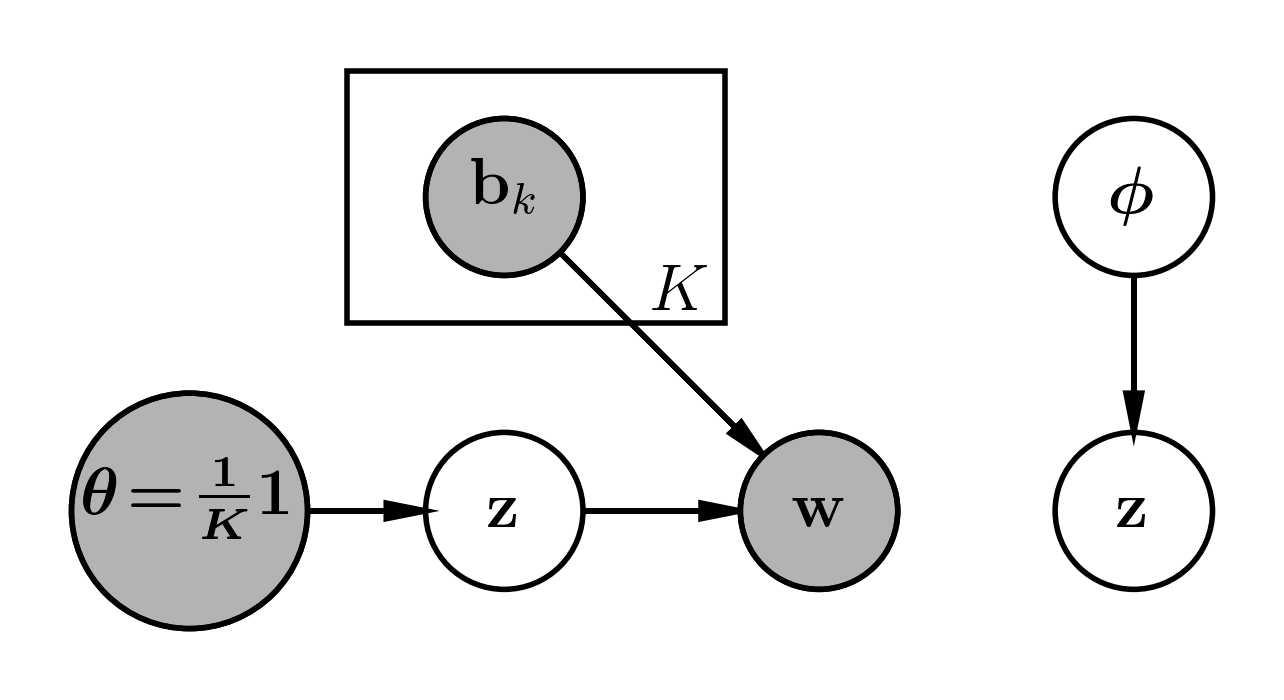
\includegraphics[width=6cm]{lda_word_embedding.png}
\caption{Inferring $\mathbf{z}$ with non-informative prior $\bm{\theta}$. The left side is the modeling and the right side is the approximation of $\mathbf{z}$}
\label{fig:lda_inference}
\end{figure}

\bibliography{lda.bib}{}
\bibliographystyle{plain}


\end{document}
